\documentclass{standalone}
\usepackage{tikz}
% create a new adjust box
\usepackage{tikzscale}
\usepackage{lscape}
\usepackage{tikz}
% use to adjust the positionS
\usetikzlibrary{positioning}
\usetikzlibrary{calc}
\tikzset{abs1/.style={xshift=3cm,yshift=2cm}}
\usetikzlibrary{shapes.geometric,arrows}
\tikzstyle{arrow}=
[thick,->,>=stealth]


\begin{document}
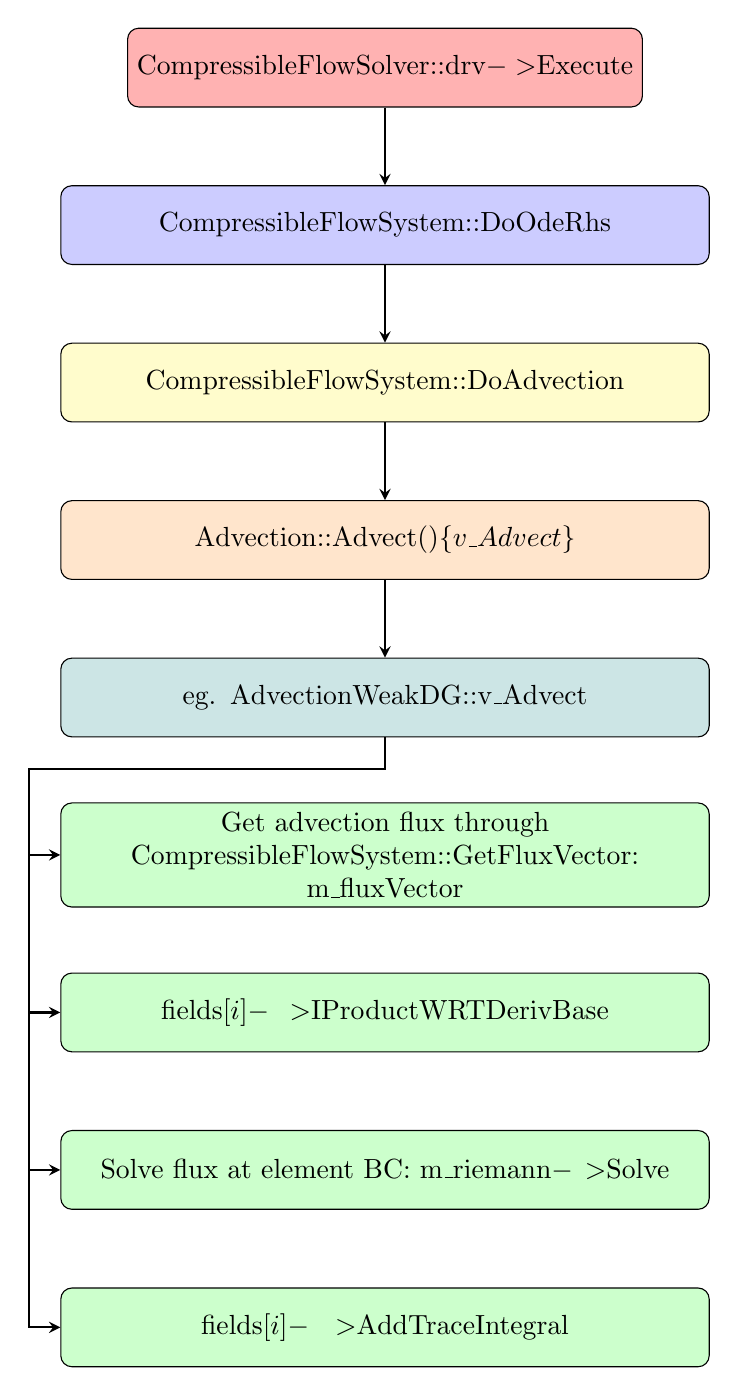
\begin{tikzpicture}[scale=0.2,node distance=2cm]
\node (A)
[rectangle,
rounded corners,
minimum width=3cm,
minimum height=1cm,
text centered,
draw=black,
fill=red!30]
{CompressibleFlowSolver::drv$->$Execute};
\node (B)
[rectangle,
rounded corners,
minimum width=8cm,
minimum height=1cm,
text width=8cm,
text centered,
draw=black,
fill=blue!20,
below of=A,
xshift=0cm,
yshift=0cm]
{CompressibleFlowSystem::DoOdeRhs};
\draw[arrow](A)--(B);
\node (C)
[rectangle,
rounded corners,
minimum width=8cm,
minimum height=1cm,
text width=8cm,
text centered,
draw=black,
fill=yellow!20,
below of=B,
xshift=0cm,
yshift=0cm]
{CompressibleFlowSystem::DoAdvection};
\draw[arrow](B)--(C);
\node (D)
[rectangle,
rounded corners,
minimum width=8cm,
minimum height=1cm,
text width=8cm,
text centered,
draw=black,
fill=orange!20,
below of=C,
xshift=0cm,
yshift=0cm]
{Advection::Advect()$\{v\_Advect\}$};
\draw[arrow](C)--(D);
\node (E)
[rectangle,
rounded corners,
minimum width=8cm,
minimum height=1cm,
text width=8cm,
text centered,
draw=black,
fill=teal!20,
below of=D,
xshift=0cm,
yshift=0cm]
{eg. AdvectionWeakDG::v$\_$Advect};
\draw[arrow](D)--(E);
\node (F_1)
[rectangle,
rounded corners,
minimum width=8cm,
minimum height=1cm,
text width=8cm,
text centered,
draw=black,
fill=green!20,
below of=E,
xshift=0cm,
yshift=0cm]
{Get advection flux through\\ CompressibleFlowSystem::GetFluxVector: \\m$\_$fluxVector};
% {m$\_$riemann$->$Solve};
\draw[arrow]($(E.south)$)--++(0,-2cm)-|($(F_1.west)+(-2cm,0)$)--(F_1.west);
% \draw[arrow](E)--(F_1);
\node (F_2)
[rectangle,
rounded corners,
minimum width=8cm,
minimum height=1cm,
text width=8cm,
text centered,
draw=black,
fill=green!20,
below of=F_1,
xshift=0cm,
yshift=0cm]
% {Get advection flux through\\ CompressibleFlowSystem::GetFluxVector: \\m$\_$fluxVector};
{fields$[i]->$IProductWRTDerivBase};
\draw[arrow]($(E.south)$)--++(0,-2cm)-|($(F_2.west)+(-2cm,0)$)--(F_2.west);
% \draw[arrow](E)--(F_2);
\node (F_3)
[rectangle,
rounded corners,
minimum width=8cm,
minimum height=1cm,
text width=8cm,
text centered,
draw=black,
fill=green!20,
below of=F_2,
xshift=0cm,
yshift=0cm]
% {fields$[i]->$IProductWRTDerivBase};
{Solve flux at element BC: m$\_$riemann$->$Solve};
\draw[arrow]($(E.south)$)--++(0,-2cm)-|($(F_3.west)+(-2cm,0)$)--(F_3.west);
% \draw[arrow](E)--(F_3);
\node (F_4)
[rectangle,
rounded corners,
minimum width=8cm,
minimum height=1cm,
text width=8cm,
text centered,
draw=black,
fill=green!20,
below of=F_3,
xshift=0cm,
yshift=0cm]
{fields$[i]->$AddTraceIntegral};
\draw[arrow]($(E.south)$)--++(0,-2cm)-|($(F_4.west)+(-2cm,0)$)--(F_4.west);
\end{tikzpicture}
\end{document}